
%(BEGIN_QUESTION)
% Copyright 2006, Tony R. Kuphaldt, released under the Creative Commons Attribution License (v 1.0)
% This means you may do almost anything with this work of mine, so long as you give me proper credit

The Foxboro model 43 pneumatic controller used a curved, clear plastic tube with a plastic ball inside as a ``null'' indicator to help the operator make ``bumpless'' transfers between auto and manual modes:

$$\includegraphics[width=15.5cm]{i01479x01.eps}$$

Give a step-by-step set of instructions to an operator for making an auto-to-manual mode transfer, using this null indicator to ensure a smooth transition between modes.

\vskip 20pt \vbox{\hrule \hbox{\strut \vrule{} {\bf Suggestions for Socratic discussion} \vrule} \hrule}

\begin{itemize}
\item{} Explain the rationale for an operator making a ``bumpless'' transfer with a controller such as this.
\item{} Describe a realistic process control scenario where a non-bumpless switch between automatic and manual modes (or vice-versa) could cause problems for the process.  If you find it helpful, make reference to a P\&ID diagram found somewhere in your homework or in your textbook.
\item{} Suppose the bias spring in this mechanism were to suddenly break.  Explain what effect(s) this fault would have on the operation of the pneumatic controller mechanism.
\item{} Suppose the controller is in automatic mode and the balance indicator ball is all the way to the left.  Describe the steps necessary to switch this controller to manual mode ``bumplessly''.
\item{} Suppose the controller is in manual mode and the balance indicator ball is all the way to the left.  Describe the steps necessary to switch this controller to automatic mode ``bumplessly''.
\end{itemize}

\underbar{file i01479}
%(END_QUESTION)





%(BEGIN_ANSWER)

Hint: the ball should be exactly centered in the tube before moving the transfer valve.

%(END_ANSWER)





%(BEGIN_NOTES)

Steps:

\begin{itemize}
\item{(1)} Adjust the ``Output Adjust'' regulator until the ball is centered
\item{(2)} Move the transfer valve from ``Auto'' to ``Manual'' mode.
\item{(3)} Adjust the ``Output Adjust'' regulator as desired to manually control the process.
\end{itemize}




\vfil \eject

\noindent
{\bf Summary Quiz:}

The purpose of the ``null indicator'' in this pneumatic controller is to:

$$\includegraphics[width=15.5cm]{i01479x01.eps}$$

\begin{itemize}
\item{} Limit the amount of output signal pressure sent to the control valve
\vskip 5pt 
\item{} Dampen the PV signal so the controller will not be affected by noise
\vskip 5pt 
\item{} Provide the operator with a way to achieve bumpless auto/manual transfer
\vskip 5pt 
\item{} Provide an easy way to adjust the proportional band of the controller
\vskip 5pt 
\item{} Provide a convenient indication of the controller's output signal pressure
\vskip 5pt 
\item{} Indicate when the setpoint and process variable signal pressures are equal
\end{itemize}


%INDEX% Control, proportional: bumpless output transfer (pneumatic)

%(END_NOTES)


